\documentclass[../thesis]{subfiles}

\begin{document}

\chapter{Implementation}


The complete eGor system is a distributed application consisting of
numerous software components running on several different
computers. To manage this complexity, the developers have attempted to
make disciplined use of best practices for web programming and to make
judicious use of a range of cutting-edge third party libraries, only
accepting those which have a record of stability and continued
maintenance.

Our complete system draws on a wide range of technologies from every
level of the software stack. This chapter provides a description of
what new components were implemented by the project's development
team, which external tools and libraries were used, and what
architectural and practical concerns factored into the selection of
these methods.



\section{Overview}

Figure \ref{fig:ImplOverview} shows a high-level schematic of the
current structure of the eGor platform. The components depicted are
divided across three different machines in the simplest scenario,
although more complex configurations are possible since all services
interact over network-ready protocols such as HTTP. These machines
are, from top to bottom
\begin{enumerate*}[label=(\roman*)]
  \item{
      the end-user's PC, where an interactive single-page browser
      application is used to interact with various eGor services
      graphically,
  }
  \item{
      a server running microservices for functions such as
      authentication, remotely accessible persistent data storage, and
      routing requests to other services and digital resources, and
  }
  \item{
      one or more machines physically connected to scientific
      equipment of interest, responsible for managing and issuing
      commands to appropriate device drivers.
  }
\end{enumerate*}

\begin{figure}
  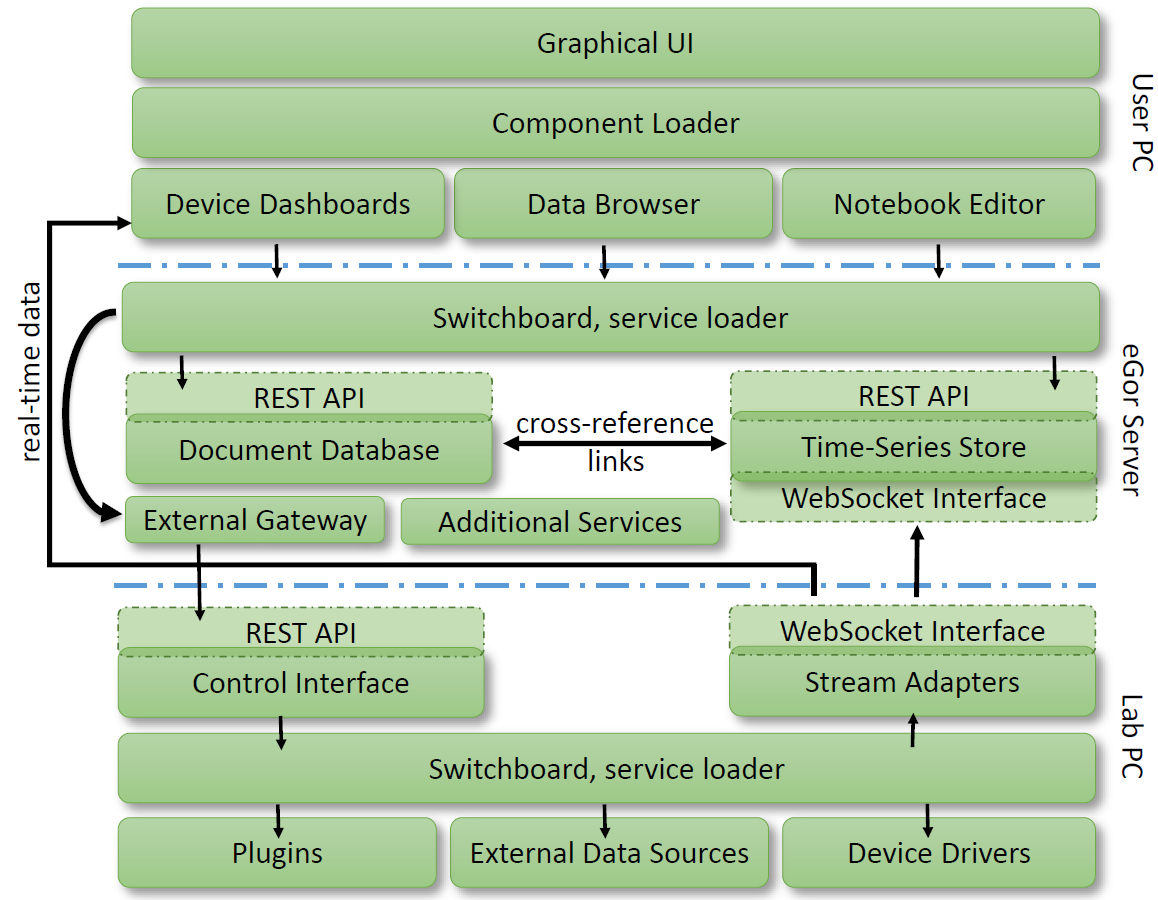
\includegraphics[width=\textwidth]{impl-overview}
  \caption{
    A high-level architectural view of the implemented eGor system,
    divided across three different machines where primary activity
    takes place: a user's machine, connected to an eGor server via a
    web browser, which issues commands to a lab PC running device
    management services to connect with lab equipment.
    \label{fig:ImplOverview}
  }
\end{figure}

This chapter will elaborate the organization and communication
strategies used to implement this framework in software, followed by a
technical discussion of each component's internals.  Other than the
in-browser graphical interface, which is written as a single-page
application in HTML5 and Javascript using the Angular framework
\cite{Angular}, the majority of the eGor web application is written in
Python \cite{Python}, making use of the mature and modern palette of
networking and communications libraries available in the language. An
important exception is found in some portions of the database access
layer, which use NodeJS \cite{NodeJS} libraries to present a simple
and effective API. Additionally, the eGor team developed a model
embedded device to help demonstrate how physical actuators and data
acquisition modules might interact with the system -- the software for
this target is written in C++. The software for all these core
components is open-source and available in several Git repositories
hosted at \url{https://github.com/egor-elab}. The diverse set of
languages used helps to demonstrate a chief strength of eGor's
microservice architecture: components are sufficiently decoupled that
they can individually be implemented in a language and style
well-suited to their unique challenges.



\section{Design principles}

Over the course of developing and refining the eGor toolchain, several
recurring patterns have emerged which seem natural fits for addressing
the application's goals and have informed subsequent iterations of the
design. This section discusses several key design patterns which have
been observed and employed throughout the code base, providing a feel
for the philosophy of the complete system before delving into
implementation details.

\subsection{Request/Response vs. Publish/Subscribe}
The most common form of high-level network traffic on the web is HTTP,
which uses request/response exchanges to pass data between hosts. For
instance, a client such as a web browser might issue an HTTP request
to a server with the contents \texttt{GET /users}, causing the server
to respond with a text payload encoding a resource named
``\texttt{users}''. The client submits user input such as form data in
a similar way (typically via an HTTP \texttt{POST} action), resulting
in an acknowledgment message from the server. This approach is
sufficiently flexible to allow for much of the broad range of content
found on the modern web, especially since servers often deliver
Javascript source code for clients to execute locally in addition to
static text documents such as HTML. Issuing commands to lab equipment
can often be modeled in a similar way: a controlling computer submits
a configuration message and the device responds with a (possibly
empty) acknowledgment that the command was received and executed.  In
many ways these operations are also analogous to the ubiquitous
programming construct of calling a subroutine, and some authors place
transactions such as HTTP actions under the umbrella of \glspl{RPC}
\cite{DBLP:journals/corr/abs-0911-4395}.

Request-and-response communication is, however, a poor fit for systems
where communications must be initiated bidirectionally, with
event-driven applications providing a key example. A typical
data-collecting lab instrument or digital microsystem produces values
in real time which must be transmitted to destinations such as
databases and display monitors at roughly the same rate as they are
captured. Implementations can still accommodate this dataflow into a
request/response framework by periodically requesting buffers from the
data source, but this approach is fraught with difficulties and is
typically complicated to use when many data sources need to be managed
simultaneously.

A more elegant design pattern for systems with soft real-time
requirements is given by the publish/subscribe approach, also
sometimes called the Observer pattern \cite{GangOfFour}. In this
scheme, a ``topic'' or ``observable'' object maintains a list of
``subscribers'', and notifies each of them when a variable of interest
changes or an event is ``published'' to the event stream. The
publish/subscribe technique has been adopted to solve software
problems like real-time data acquisition as well as for building
``reactive'' applications such as user interfaces and games, where
graphical interfaces are expected to react seamlessly to event streams
such as user input and network communications. eGor adopts this
pattern for both these use cases, treating data collection devices as
publishers of streams of data fragments which may be subscribed to by
other services or graphical interfaces throughout the system.

\subsection{Dynamic loading}
One of the chief observations underpinning eGor's design is that
researchers' needs are too diverse and rapidly changing to be
satisfactorily addressed by a single rigidly constructed
application. The implementation effort has therefore focused on
constructing a core infrastructure which allows future developers to
easily integrate new functionality without disturbing the system's
overall operation. Each major component of eGor allows its users to
load new extensions at runtime. The core subsystems each specify an
interface for how a module should allow itself to be installed and
expose its functionality to the network, and otherwise
community-contributed extensions are not required to depend on eGor
APIs or even to be written in the same programming language as the
rest of the framework.

In addition to being an essential part of the daily workflow for
eGor's developers, a distributed version control system (namely Git
\cite{Git}) provides a runtime mechanism for achieving ths dynamic
loading functionality. Git was designed to allow many programmers to
collaborate on a software project, share contributions remotely, and
review and revert changes. Importantly, Git is distributed in the
sense that each user may maintain an independent timeline of the
history of the code base on a private computer, with or without
network connectivity, sharing or publishing changes in a peer-to-peer
fashion if and when they choose.

An example of the dynamic loading process is illustrated in figure
\ref{fig:DynamicLoading}. The following sequence of steps describes
how, for instance, the device management system might \glspl{lazyLoad} a
device driver, waiting to download and install the appropriate code
until the device has been physically connected to a given host machine
for the first time. Here the phases are listed with the same numbering
as in figure \ref{fig:DynamicLoading}.

\begin{enumerate}
  \item{
      A client service attempts to access functionality on another
      service which is not presently running, or explicitly requests for
      a new service to be loaded. In this case, the client is a service
      responsible for enumerating the serial ports available on the
      system and attempting to retrieve identifying information from
      connected devices, and its request for a device driver includes
      identifying information but may not name the driver explicitly.
  }
  \item{
      The ``service-hosting service'', responsible for managing
      dynamically loaded programs, queries a database of service
      information to determine where it can download the requested
      code. The database responds with a \gls{URI} specifying either a
      direct link to the necessary files or a Git repository.
  }
  \item{
      The service-hoster downloads the module, possibly from an
      internal server or from a publically hosted location such as
      Github \cite{Github}, and executes necessary startup
      routines. If the service-hoster determines that the service is
      already loaded, it instead checks if an updated version exists
      and provides the client with the option to download and use the
      new version. eGor services are expected to implement a common
      interface of setup, start, stop, and cleanup scripts so that the
      service-hoster can install and run them automatically. The
      service-hoster also indicates to the new service instance how it
      can communicate with the system switchboard responsible for
      triggering the download.
  }
  \item{
      Once the dynamically loaded device driver is live, it registers its
      public \gls{API} with the switchboard, at which point the
      driver's functionality is available for other services to use.
  }
  \item{
      The switchboard completes any pending procedure calls requested
      by the client service, and routes subsequent requests to the
      appropriate service.
  }
\end{enumerate}

A similar procedure is employed for several other
subsystems, such as loading new user interface components or adding
new waveform generation routines to our real-time electrochemical
interrogation platform.


\begin{figure}
  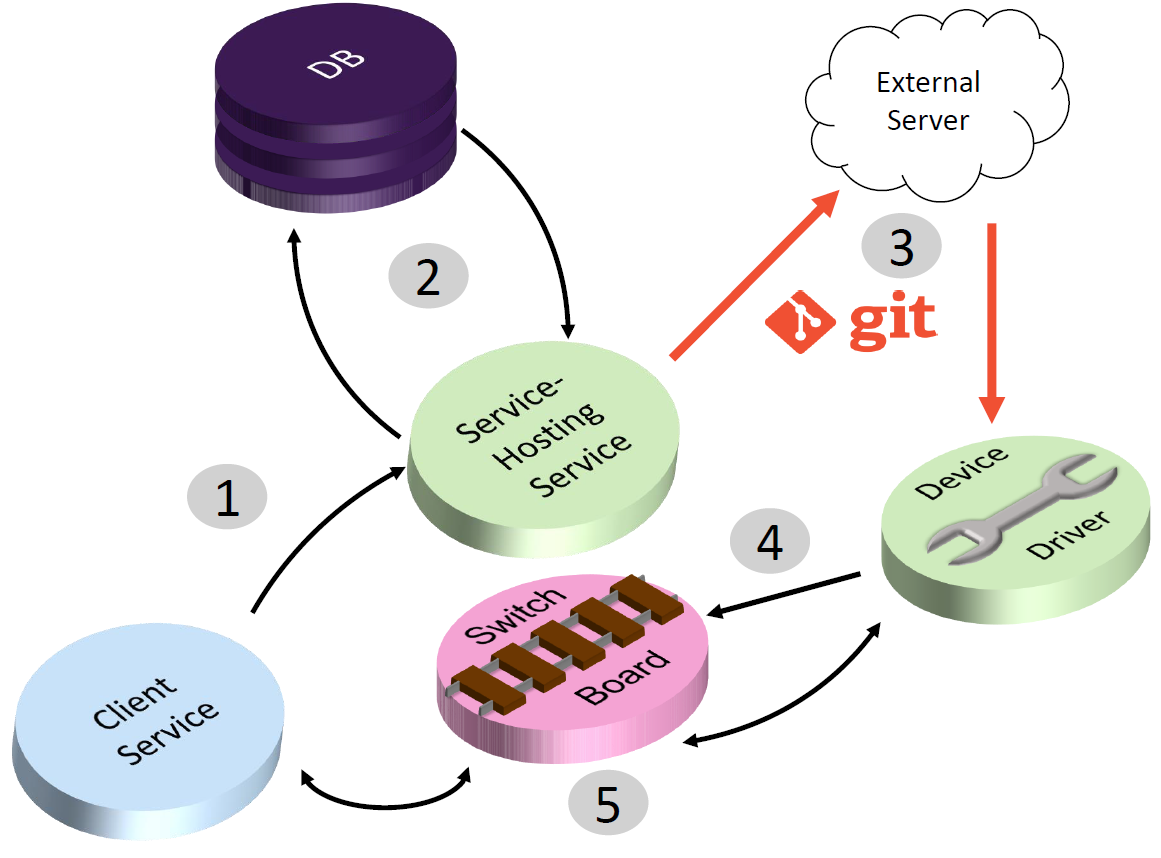
\includegraphics[width=\textwidth]{dynamic-loading}
  \caption{
    Phases of the dynamic loading process for downloading and
    installing a user-defined device driver at runtime. The
    service-hosting service and the services it hosts (green)
    run on the same physical hardware, whereas each other service may
    be on a different device connected via the Internet.
    \label{fig:DynamicLoading}
  }
\end{figure}

\subsection{API/structure isomorphism}



\section{Service interconnect}

As described in Chapter 3, the microservice architectural pattern
provides a strategy for compartmentalizing the development effort,
promoting modularity of design, allowing for future customization and
extension, and building a system that employs many different software
technologies and physical machines. However, communication between
microservices involves some challenges compared to traditional
architectures and relies on several recently emerged web technologies
to allow services to locate and use one another. Nonetheless,
the microservice approach pairs well with eGor's high-level goals and
has enabled us to build a flexible and sophisticated system.

\subsection{REST APIs}



\subsection{WAMP Routing}
The \gls{WAMP} protocol and software stack described by Crossbar.io
\cite{CrossbarIO} provides a set of capabilities which are a good
match for our application, including built-in support for routing
remote procedure calls between any two connected services and
bidirectional ``publish/subscribe''-style message passing
\cite{WAMP}. The protocol was explicitly designed to simplify the
implementation of \gls{IoT} applications, especially those with
service-oriented architectures that span multiple devices of different
types.


\section{User interface}

\subsection{Thin-client design}

\subsection{Angular 2}


\section{Database management}

\subsection{NoSQL / schemaless}
Traditional web applications typically use relational databases for
persistent data storage, querying and assemblying them using \gls{SQL}

\subsection{LoopBack}

\subsection{HDF5}
Although NoSQL databases such as MongoDB provide a flexible solution
for persistent storage of complex document-like data, they are
ill-suited for efficiently querying large array-like scientific data
sets.   HDF5 is a technology for manipulating multidimensional
time-indexed formats that has seen strong adoption in the finance, machine
learning, and data science fields in recent years \cite{HDF5}. The
open source working group responsible for developing the HDF5
specification has also provided a Python web server for storing
datasets and presenting them as network resources, which includes a
reference implementation of a REST API for remotely manipulating
and extracting subsets of datasets.


\section{Device management}

\subsection{Enumeration}


\subsection{Protocol codecs}
One of the most important capabilities of the eGor system is its
ability to connect to computer-controlled lab equipment. Scientific
processes often involve a wide range of legacy instruments which use
different communication protocols and data formats. Rather than
attempting to provide individual drivers and protocol translators for
the many devices that our future users may need, we have constructed a
Python library of simple   which can be connected into more elaborate
protocol stacks.




\end{document}
